\section{Modelos de Plasticidade}

Como explicado na seção~\ref{section_plasticidade}, a STDP foi a primeira forma de plasticidade observada e tem sido amplamente
utilizada como a principal regra de aprendizado em modelos computacionais de aprendizado, muito embora seu grau de importância com
relação a outras formas de plasticidade no cérebro ainda não é completamente compreendido~\cite{feldmanSpike2020}.

\begin{equation}
\label{eq_stdp1}
\frac{dw}{dt} = 
\begin{cases}
      A_{+} \exp(\frac{t_{\text{pré}} - t_{\text{pós}}}{\tau_{+}}) & \text{se $t_{\text{pré}} \le t_{\text{pós}}$}\\
      -A_{-} \exp(-\frac{t_{\text{pré}} - t_{\text{pós}}}{\tau_{-}}) & \text{se $t_{\text{pré}} > t_{\text{pós}}$}\\
\end{cases}
\end{equation}

A Equação~\ref{eq_stdp1} representa como o peso da sinapse, $w$, varia de acordo com a diferença do tempo de disparos dos
neurônios pré- e pós-sináptico, onde $\tau_{\pm}$ são as constantes de tempo. Se o disparo pré-sináptico ocorre antes do disparo
pós-sináptico ($t_{\text{pré}} \le t_{\text{pós}}$), significa que há uma correlação entre os dois disparos, e a sinapse é potencializada de
acordo com uma regra exponencial, quanto mais próximos em tempo forem os disparos, mais relevante é essa correlação. Caso o
neurônio pós-sináptico dispare antes do pré-sináptico, então ele foi ativado por algum outro motivo e não há relação com o disparo
pré-sináptico, portanto a sinapse é deprimida~\cite{yamazakiSpiking2022}.

A STDP, como todas as formas de plasticidade hebbiana, é instável~\cite{gerstnerSpiking2002}. No trabalho
de~\cite{zenkeDiverse2015}, dois tipos de plasticidade não hebbiana foram utilizados para estabilizar a rede: em baixas
frequências de disparos, a potenciação induzida por transmissor vai contra a Depressão de Longa Duração (LTD), evitando que a rede
inteira caia em silêncio por constante diminuição da força das sinapses; em altas frequências de disparos, a depressão
heterossináptica garante que algumas sinapses não se tornem absurdamente fortes e, por consequência, a única parte ativa da rede.

A Equação~\ref{eq_stdp1} também pode ser melhorada de forma a se tornar mais estável, como demonstra a Equação~\ref{eq_stdp2}.

\begin{equation}
\label{eq_stdp2}
\begin{cases}
    A_{+}(x) = \eta_{+} \exp(-w)\\
    A_{-}(x) = \eta_{-} \exp(w)\\
\end{cases}
\end{equation}

Aqui, o termo $A_{\pm}$, que é responsável por escalar a mudança de peso, é tornado dependente do peso para que os valores do peso
não aumentem demais ou diminuam demais. O termo $\eta_{\pm}$ é um parâmetro que controla a taxa de aprendizado.

Outra inconsistência biológica desse modelo é que um neurônio não é capaz de memorizar todos os tempos de disparo. Para isso, é
introduzido o conceito de um rastro do disparo, $x$.

\begin{equation}
\label{eq_stdp3}
\frac{dw}{dt} = A_{+} x_{\text{pré}} \delta_{\text{pós}} - A_{-} x_{\text{pós}} \delta_{\text{pré}}
\end{equation}

De acordo com a Equação~\ref{eq_stdp3}, caso haja um disparo no neurônio pós-sináptico (indicado por $\delta_{\text{pós}}$), o peso da
sinapse é potencializado de acordo com o rastro do disparo do neurônio pré-sináptico ($x_{\text{pré}}$). Caso haja um disparo no
neurônio pré-sináptico (indicado por $\delta_{\text{pré}}$), o peso da sinapse é deprimido de acordo com o rastro do disparo do neurônio
pós-sináptico ($x_{\text{pós}}$).

O rastro de disparo é atualizado de acordo com a Equação~\ref{eq_stdp4}.

\begin{align}
\label{eq_stdp4}
\frac{dx_{\text{pré}}}{dt} &= -\frac{x_{\text{pré}}(t)}{\tau_{+}}+\delta(t)\\
\frac{dx_{\text{pós}}}{dt} &= -\frac{x_{\text{pós}}(t)}{\tau_{-}}+\delta(t)
\end{align}

Aqui, $x_{\text{pré}}$ e $x_{\text{pós}}$ são os rastros de disparo dos neurônios pré- e pós-sináptico, respectivamente, e começa
em zero. Caso haja um disparo no tempo $t$, o rastro de disparo é incrementado em um e decai exponencialmente com uma constante de
tempo $\tau_{\pm}$. Esse modelo de plasticidade é chamado de STDP estável (S-STDP)~\cite{paredes-vallesUnsupervised2018} A
Figura~\ref{fig_stdp} ilustra o funcionamento da STDP entre dois modelos de neurônio.

\begin{figure}[!ht]
\caption{STDP entre dois neurônios.}
\centering{
\parbox{12cm}{
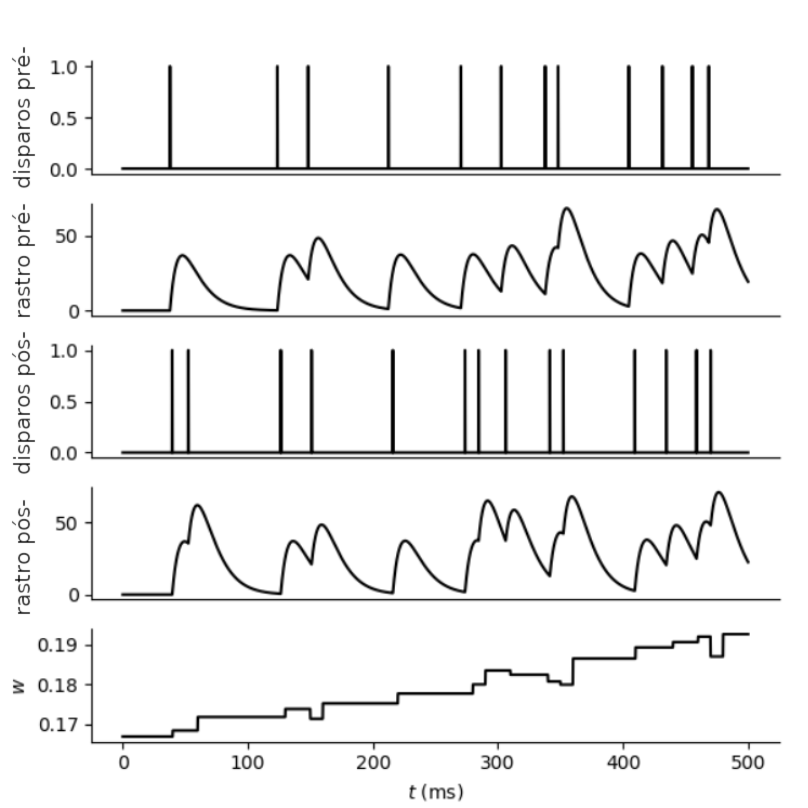
\includegraphics[width=12cm]{figuras/stdp.png}\label{fig_stdp}
\fonte{\cite{yamazakiSpiking2022}. Modificada pelo autor.}}}
\end{figure}



